%%
% 第三章：基于 π0.5 的抓取策略训练与实机部署
%%

\chapter{基于 $\pi_{0.5}$ 的抓取策略训练与实机部署}
\label{chap:pi05-franka}

第二章完成了机械臂与 LeRobot 通用接口的打通（T1）以及桌面抓取示教数据的标准化采集与组织（T2）。
本章对应设计任务 T3（$\pi_{0.5}$ 模型迁移与变体改进）与 T4（实机闭环部署与在线执行策略对比）。设计目标有两个：首先，将 $\pi_{0.5}$ 预训练权重迁移至桌面抓取任务并完成全量微调基线，进而提出冻结骨干与短期记忆两项结构变体以改善小样本条件下的性能与效率；其次，通过受控对比实验量化不同在线闭环策略对同一模型权重在接触敏感任务上的性能影响。具体而言，本章重点说明：$\pi_{0.5}$ 模型\cite{black2025pi05} 的核心原理与为何其适合迁移到桌面抓取任务；本文如何将双视角观测、八维状态/动作以及自然语言任务提示映射到 OpenPI 训练接口，并基于自采数据集完成微调训练；训练后模型在不同在线执行方式下呈现的显著性能差异，尤其是逐段闭环推理带来的成功率提升；以及结合本文改动与实验观察，对冻结骨干与短期记忆等模型变体的定量对比与行为分析。

需要指出的是，本文的算法贡献并非简单复现已有 $\pi_{0.5}$ 结果，而是将其从原论文面向移动双臂家庭机器人、长时程多阶段任务的设定，迁移到静态桌面抓取这一更聚焦但接触精度要求更高的场景中。
为此，本文完成了数据接口重构、训练配置适配、在线执行闭环设计与行为层面的现象分析，
从而形成“硬件接入--示教采集--策略训练--实机部署”的完整毕业设计闭环。

\section{$\pi_{0.5}$ 的核心原理框架}
\label{sec:pi05-core}

\subsection{从 VLA 到分层推理}

视觉--语言--动作模型（Vision-Language-Action, VLA）试图直接学习从观测与语言指令到机器人动作的映射。对单步或动作块预测而言，其基本目标可写为
\begin{equation}
  \max_{\theta}\;
  \mathbb{E}_{(\mathbf{a}_{t:t+H},o_t,\ell)\sim\mathcal{D}}
  \log \pi_{\theta}(\mathbf{a}_{t:t+H}\mid o_t,\ell),
  \label{eq:pi05-il}
\end{equation}
其中 $o_t$ 包含时刻 $t$ 的多相机图像与机器人本体状态，$\ell$ 为自然语言任务指令，$\mathbf{a}_{t:t+H}$ 表示长度为 $H$ 的动作块。与传统仅依赖低维状态的行为克隆不同，VLA 同时利用视觉与语言信息，使策略具备更强的任务条件表达能力与跨对象泛化潜力\cite{black2024pi0}。

$\pi_{0.5}$ 的关键思想在于：将高层语义推理与低层动作生成统一到同一个多模态序列建模框架中，而不是单纯把“图像+文本”直接映射为动作。传统的端到端模仿学习策略往往直接输出控制量，虽然在单一任务上可以工作，但一旦任务中包含“先观察目标、再对准、再夹取、再搬运”的多阶段结构，纯低层策略往往难以显式表达当前子目标。$\pi_{0.5}$ 试图解决的正是这一问题：它既保持了 VLA 对视觉和语言的理解能力，又把“当前应该做什么”编码成显式语义中间层，使动作生成不再完全依赖隐式内部状态。

原论文将模型分解为高层子任务推断与低层动作预测两部分，其联合分布可写为
\begin{equation}
  \pi_{\theta}(\mathbf{a}_{t:t+H},\hat{\ell}\mid o_t,\ell)
  =
  \pi_{\theta}(\hat{\ell}\mid o_t,\ell)\;
  \pi_{\theta}(\mathbf{a}_{t:t+H}\mid o_t,\hat{\ell}),
  \label{eq:pi05-factor}
\end{equation}
其中 $\hat{\ell}$ 表示模型根据当前场景与高层任务自动生成的语义子任务，例如“抓住苹果”“移动到桌面左上角”等。该结构的意义在于：模型可以先决定“当前最合适做什么”，再决定“具体如何做”，从而把长时程任务分解成若干更稳定的局部动作过程。这种思路与语言模型中的链式推理存在相似性，但 $\pi_{0.5}$ 将其落到了机器人可执行的动作闭环中\cite{black2025pi05}。从控制角度看，式~\eqref{eq:pi05-factor} 也意味着模型把任务分解误差与动作跟踪误差在建模层面分离开来：高层语义负责减少“做错事”的风险，低层动作负责减少“做不准”的风险。

对于本文的桌面苹果抓取任务，虽然任务长度远短于原论文中的“整理厨房”“铺床”等家庭长任务，但接近目标、夹取接触、抬升确认、放置到指定区域依然天然构成了一个多阶段操作链。因此，$\pi_{0.5}$ 的分层思想依旧具有价值：高层语义可帮助策略在“寻找目标--对准抓取--完成搬运”之间切换，而低层动作块则负责生成连续、可执行的关节与夹爪指令。特别是在苹果这类易滚动、易滑移物体的抓取中，若没有对子目标的良好组织，低层策略很容易把“接近目标”和“稳定夹持”混为一个不可分的黑盒过程，导致接触阶段误差被快速放大。

\subsection{统一多模态序列建模}

$\pi_{0.5}$ 的第二个关键点，是它并没有为“看图”“理解语言”“预测子任务”“输出动作”分别设计彼此割裂的模型，而是试图把这些信息都放到一个统一的序列建模框架中。其底层做法是：将图像 patch、文本 token、机器人本体状态以及动作相关表示映射到同一 Transformer 中，通过注意力机制建立跨模态关联。这样一来，模型在看到第三人称图像中的苹果、腕部相机中的夹爪位置以及文本提示“抓取苹果并放到左上角”时，可以在统一特征空间里决定当前最相关的信息组合。

从模型设计看，$\pi_{0.5}$ 并不是简单把所有 token 串在一起做标准因果注意力，而是使用了前缀--后缀式的注意力组织。图像、语言提示以及部分状态信息作为前缀，允许在前缀内部进行充分的信息交互；动作相关 token 则作为后缀，在访问前缀条件信息的同时保持适合动作生成的依赖结构。这样的设计有两个直接好处：一方面，动作生成不再只依赖某一个单独编码后的观测向量，而是依赖整个多模态上下文序列，充分利用视觉语义上下文；另一方面，同一个主干既可以输出文本型子任务，也可以为后续动作专家提供条件特征，便于统一高层与低层推理。

对本文任务而言，这种统一建模尤其重要。由于桌面抓取同时依赖全局视角与局部手眼视角，如果采用两套完全分离的感知链路，系统往往会面临信息对齐复杂、训练目标割裂的问题。而在 $\pi_{0.5}$ 框架中，第三人称图像更偏向提供目标位置和放置区域的全局语义，腕部图像更偏向提供夹取局部几何与接触反馈，两者都被放入同一个条件上下文中，因此更适合学习“先粗定位、再精对准”的策略模式。

\subsection{主干网络与动作专家}

在结构上，$\pi_{0.5}$ 建立在 $\pi_{0}$\cite{black2024pi0} 之上，延续了“视觉语言主干 + 动作专家（action expert）”的设计。主干部分继承预训练视觉语言模型的表征能力，其核心由 SigLIP 视觉编码器和 Gemma 语言模型骨干组成；图像被切分为 patch token，自然语言指令被编码为文本 token，而机器人状态与动作则通过专门的投影与编码方式进入同一 Transformer 序列中\cite{beyer2024paligemma}。这样做的本质，是把机器人控制问题转化为统一的多模态序列建模问题。

与纯文本自回归模型不同，机器人策略不仅要输出语义 token，还要输出连续动作。为此，$\pi_{0.5}$ 在主干之外引入更小的动作专家模块，对动作块进行专门建模。动作专家的作用可以概括为两点。首先，主干网络保留语言与视觉理解能力，动作专家则专注于生成高精度、低时延的连续控制量，实现语义推理与连续控制的分离；其次，若直接以离散动作 token 自回归逐个采样，实机部署时延较大，动作专家将动作块视为连续变量分布，能以更少的推理步数生成整个动作序列，提高在线推理效率。

相比之下，$\pi_{0.5}$ 相对于 $\pi_{0}$ 有两处重要改变。首先，机器人状态可以作为离散语言 token 的一部分输入，而非仅作为连续后缀输入；其次，在动作专家中使用自适应归一化（adaRMSNorm）的方式注入 flow matching 时间步，使每一层动作专家都能感知当前的去噪阶段。本文在训练配置中启用了上述路径，确保模型结构接近论文原意的 $\pi_{0.5}$ 设计。

\subsection{动作专家中的 Flow Matching 机制}

动作专家与 flow matching 的结合，是 Pi 系列模型区别于许多传统 VLA 的核心创新之一。其出发点在于：离散 token 对大规模预训练很友好，但真实机器人控制需要的是连续、平滑、低延迟的动作输出；如果完全依靠离散动作 token 自回归采样，不仅推理速度受限，而且连续控制精度也可能受动作量化误差影响。Pi 系列的关键设计，就是在保留大模型主干语义能力的同时，用一个更小、更专门化的动作专家来建模连续动作分布\cite{black2024pi0,black2025pi05}。

设真实动作块为 $\mathbf{a}_{t:t+H}$，噪声为 $\boldsymbol{\omega}\sim\mathcal{N}(0,I)$，时间变量为 $\tau\in[0,1]$，则 flow matching 中的中间变量可写为
\begin{equation}
  \mathbf{x}_{\tau}
  =
  \tau\boldsymbol{\omega} + (1-\tau)\mathbf{a}_{t:t+H}.
  \label{eq:flow-interp}
\end{equation}
其直观含义是：当 $\tau$ 接近 $1$ 时，$\mathbf{x}_{\tau}$ 更接近纯噪声；当 $\tau$ 接近 $0$ 时，$\mathbf{x}_{\tau}$ 更接近真实动作。动作专家并不直接回归最终动作，而是学习一个向量场，把当前的噪声化动作逐步“拉回”到真实动作块所在的分布流形上。若记目标向量场为
\begin{equation}
  \mathbf{u}_{\tau}
  =
  \boldsymbol{\omega}-\mathbf{a}_{t:t+H},
  \label{eq:flow-vector}
\end{equation}
则模型的任务可以理解为：在给定观测条件 $o_t$、任务提示 $\ell$ 以及当前中间状态 $\mathbf{x}_{\tau}$ 的情况下，预测一个足以将当前样本推向真实动作的连续更新方向。

这种设计相比直接回归动作块，具有三方面优势。第一，表达能力更强。对于多峰或接触敏感的动作分布，直接回归往往倾向于输出平均动作，而 flow matching 更适合刻画连续动作分布的形状。第二，推理效率更高。模型不需要逐 token 自回归采样完整动作序列，而是通过少量迭代积分生成整段动作。第三，与大模型主干天然解耦。动作专家可以比主干小很多，只负责连续控制这一件事，因此既保留了主干的视觉语言能力，又避免把所有控制负担都压到超大参数主干上。

Pi 系列的一个关键工程点是如何将时间步 $\tau$ 注入动作专家。$\pi_{0}$ 主要通过将时间信息与动作 token 混合后再输入动作分支；而 $\pi_{0.5}$ 更进一步，采用自适应归一化的方式注入时间条件：独立的时间多层感知机（MLP）生成时间嵌入，作为每一层动作专家自适应 RMS 归一化的条件输入，而非简单拼接到动作 token 后。这一设计使时间步信息对整条去噪轨迹的调制更加稳定，也更符合“动作专家专门负责连续流场生成”的定位。

从本文桌面抓取任务看，flow matching 的价值尤其体现在接近--闭合--抬升这类短时连续接触动作中。若动作输出过于离散，夹爪闭合时机、抬升速度和末端姿态变化都容易产生不连贯现象；而 flow matching 生成的连续动作块更容易保持轨迹平滑。进一步结合本文后续的分段闭环执行策略，可以把这种连续动作块理解为“局部时间窗内的平滑控制建议”，再通过频繁重推理不断修正，从而兼顾了平滑性与反馈性。

\subsection{离散动作预训练与连续动作后训练}

$\pi_{0.5}$ 训练流程的第二个核心，是离散动作表示与连续动作表示的结合。原论文在预训练阶段使用 FAST 动作离散化\cite{pertsch2025fast}，将动作块编码为离散 token，从而能够用标准自回归 next-token prediction 的方式大规模高效训练；而在后训练阶段，则引入 flow matching\cite{lipman2022flowmatching} 风格的连续动作生成机制，以获得更适合实时控制的连续输出。
更具体地说，$\pi_{0.5}$ 不是在预训练阶段就完全依赖连续动作建模，而是先利用离散动作 token 获得高效、稳定的大规模训练，再在后训练阶段加入动作专家与连续动作目标。这样做的原因是：离散 token 训练与大模型生态更加兼容，便于复用已有视觉语言主干；而连续动作建模则更适合最终实机部署。原论文形式化地将总目标写成文本交叉熵损失与连续动作场回归损失的加权和\cite{black2025pi05}。对本文而言，这一机制的意义在于：训练阶段能够继承预训练 VLM 在语义与视觉上的能力；部署阶段能够直接输出连续关节/夹爪动作块，避免全自回归动作采样导致的时延；此外，通过动作块预测，使控制器在短时域内保持动作连续性与平滑性。

\subsection{异构数据协同训练的意义}

$\pi_{0.5}$ 之所以区别于传统桌面行为克隆策略，不只因为模型结构更大，更重要的是其协同训练（co-training）思想。原论文并不是只用目标机器人自己的示教数据训练策略，而是把多种来源的数据放进同一个训练食谱中，包括：不同机器人本体的数据、跨场景的数据、高层语义子任务标注、网页图文数据以及目标平台上的后训练数据\cite{black2025pi05}。这种思路的直接收益是：即便目标场景上的机器人数据规模有限，模型依然可以从外部多模态知识中继承对象识别、语言对齐与任务分解能力。

本文的桌面抓取实验仅使用了 30 条自采轨迹，规模远小于原论文数百小时级别的数据量，因此更能体现 $\pi_{0.5}$ 这种”先借助大模型与异构数据获得通用能力，再用小规模专用数据做任务特化”的价值。针对小样本、接触敏感的桌面任务特性，本文提出了冻结视觉语言骨干与短期记忆两项模型结构改进，其原理与实现详见第四章。

\section{面向桌面抓取的模型适配与训练实现}
\label{sec:pi05-training}

\subsection{任务观测与动作空间重定义}

原始 $\pi_{0.5}$ 论文面向带移动底盘、升降机构与双臂夹爪的家庭服务机器人，其状态与动作空间维数达到 $18\sim19$ 维，且在高层推理时会使用四路相机，在低层动作推理时使用前向相机与双腕相机\cite{black2025pi05}。本文场景则聚焦于静态单臂桌面抓取，其控制对象与观测形式更紧凑，因而必须进行接口层与数据层的重新定义。

本文在训练配置中将数据重排为如下结构：图像输入将第三人称相机映射为全局视角（base）、腕部相机映射为手眼视角（wrist），状态输入使用 observation.state 作为低维本体状态，动作监督使用 action 作为策略目标，语言提示使用数据集中的任务描述作为文本输入。

结合第二章的数据集定义可知，本文任务中的 state 与 action 均为八维向量：前七维对应 弗兰卡 七轴关节，第八维对应夹爪开合量。这样一来，本文的动作空间既保留了夹取任务所需的末端开合信息，又避免了在小数据场景下额外建模底盘与多臂协调，从而使训练重点聚焦到“桌面目标定位、抓取对准、夹紧抬升与搬运放置”这几个关键环节。

这种改写的价值在于：虽然本文采用的是 $\pi_{0.5}$ 的总体思路，但并未机械照搬原论文的机器人输入格式，而是将观测--动作接口完全纳入 OpenPI 可消费的通用数据范式。这正是第二章工作的算法侧落点：没有前面的接口统一与数据规范化，就无法把原本服务于通用机器人 VLA 的训练框架直接用于本平台实机任务。

\subsection{训练配置与关键超参数}

表~\ref{tab:pi05-train-config} 汇总了本文桌面苹果抓取任务的主要训练设置。训练配置整体遵循”加载 $\pi_{0.5}$ 基础权重，在本地数据集上进行任务微调”的思路，既保留了原模型动作块预测的优点，也针对桌面任务做了更紧凑的时域设置。

\begin{table}[htbp]
  \centering
  \small
  \caption{苹果抓取训练配置}
  \label{tab:pi05-train-config}
  \begin{tabular}{>{\raggedright\arraybackslash}p{3.8cm}>{\raggedright\arraybackslash}p{8.0cm}}
    \toprule
    配置项 & 取值与说明 \\
    \midrule
    模型类型 & $\pi_{0.5}$（动作块长度 32，最大 token 长度 200） \\
    数据集 & 自采桌面抓取数据集，本地加载 \\
    图像映射 & 第三人称相机 $\rightarrow$ 全局视角，腕部 $\rightarrow$ 手眼视角 \\
    状态 / 动作 & 8 维关节与夹爪状态 / 8 维关节与夹爪动作 \\
    语言提示 & 数据集任务描述字段 \\
    预训练权重 & 加载 $\pi_{0.5}$ 基础权重 \\
    归一化统计量 & 复用预训练资产中的归一化参数 \\
    批大小 & 4 \\
    数据加载线程数 & 2 \\
    训练步数 & 50,000 \\
    模型保存间隔 & 每 10,000 步 \\
    \bottomrule
  \end{tabular}
\end{table}

其中有三项设置需要重点提及。

在时域设置上，本文将动作块长度设为 $32$。与原论文更长的动作视界相比，更短的动作块有利于减少单次预测覆盖的开环时间，降低接触误差积累，同时在后续部署中更容易结合”执行一部分动作后重新观测再推理”的策略。

在序列容量上，最大 token 长度设为 200。虽然本文任务文本提示较短，但由于 $\pi_{0.5}$ 会把状态与多模态条件统一编码到序列中，保留较大的 token 容量可避免在迁移过程中因输入裁剪而损失条件信息。

在参数初始化上，训练配置加载已有的 $\pi_{0.5}$ 基础权重，再结合本文任务数据进行继续训练。对于仅有 30 条示教数据的小规模数据集而言，这是获得可用性能的关键前提：视觉主干与语言主干提供通用感知能力，动作专家与相关层在任务数据上完成针对性调整。

\subsection{本文对 $\pi_{0.5}$ 的适配工作}

本文对 $\pi_{0.5}$ 的工作并非简单的”换数据训练”，而是围绕桌面抓取场景完成了四个层面的针对性适配。

首先是平台适配。将单臂与二指夹爪的八维状态/动作与 LeRobot 标准数据集字段对齐，再进一步映射到 OpenPI 的多模态输入接口，使训练框架可直接消费第二章构建的数据集。

其次是观测适配。从原始移动机器人多相机设定收缩到”第三人称 + 腕部相机”的双视角组合，保留对目标定位和精细接触都最关键的视觉信息，同时降低输入维度的冗余。

再次是部署适配。不直接照搬整段动作块开环执行，而是针对真实接触任务设计了更紧凑的”短时执行 + 重观测重推理”闭环策略（详见第\ref{sec:pi05-deploy}节），大幅提升接触敏感阶段的在线修正能力。

最后是评估适配。将原论文面向开放家庭场景的泛化指标转换为本文任务更关心的抓取成功率、掉落/滑移现象以及失败后的再搜索能力，形成可定量对比的实验基准。

\section{在线推理执行策略与实机效果分析}
\label{sec:pi05-deploy}

\subsection{两种部署方式的差异}

训练完成后，本文分别使用异步远端推理与分段同步闭环两种部署方式进行实机测试。两者都通过 WebSocket 与 OpenPI 远端推理服务通信，并向机械臂发送关节与夹爪指令，但其控制闭环方式明显不同。

异步远端推理采用推理线程与控制线程解耦的方式：推理线程不断发送最新观测并获取新的动作块，控制线程则以固定频率执行“当前最新的有效动作”。如果某些动作在推理返回时已经过期则直接丢弃。这种设计在理论上可以提高系统利用率，但也意味着机器人在执行阶段可能使用的是一段并非基于最新视觉反馈重新规划得到的动作序列，执行偏长时开环。

分段同步闭环则采用截然不同的方式：每次先读取一次机器人观测，推理得到一整个动作块后，仅截取其中一小段（约 8 步）执行，执行完成后立刻重新读取新观测并再次推理。若系统控制频率取 $30~\mathrm{Hz}$，则一次执行窗口大约只覆盖
\begin{equation}
  \Delta t \approx \frac{8}{30}\ \mathrm{s} \approx 0.27\ \mathrm{s},
\end{equation}
这使得策略以“短时开环 + 高频重规划”的方式运行。虽然总推理次数增多，但它显著增强了接触任务中的在线修正能力。

\begin{table}[htbp]
  \centering
  \small
  \caption{两种部署方式对比}
  \label{tab:deploy-compare}
  \begin{tabular}{>{\raggedright\arraybackslash}p{3.2cm}>{\raggedright\arraybackslash}p{3.6cm}>{\raggedright\arraybackslash}p{3.8cm}>{\raggedright\arraybackslash}p{2.8cm}}
    \toprule
    部署方式 & 控制方式 & 典型行为特征 & 实验现象 \\
    \midrule
    异步远端推理 & 异步推理 + 固定频率执行最新动作块 & 动作可能在返回时部分过期，执行更偏开环 & 成功率很低，约 $5\%$，苹果常滑走 \\
    分段同步闭环 & 同步分段推理，每次只执行动作块的一小段 & 高频“观测--执行--再观测--再执行”闭环 & 成功率接近 $100\%$，抓取稳定显著提升 \\
    \bottomrule
  \end{tabular}
\end{table}

\subsection{成功率差异的原因分析}

本文实验中最突出的现象是：采用异步远端推理时，抓取成功率仅约为 $5\%$；而改用分段同步闭环后，成功率大幅提升，接近 $100\%$。
二者使用的是同一个训练后的模型，因此这一差异主要不是由模型参数本身导致，而是由在线闭环方式决定的。

结合任务过程，可以将原因概括为以下三点。

首先，桌面抓取是强接触敏感任务，不能长时间开环。苹果表面光滑、受力后易滚动或侧滑，机械臂在接近苹果、闭合夹爪以及抬升初期这几个阶段，对末端相对位姿误差极为敏感。若模型依据稍早的观测生成一整段动作，而环境在执行中已经发生细小变化（例如苹果被碰动、夹爪接触点偏移），则后续尚未执行完的动作就会迅速失效。异步方式虽然也会丢弃明显过期动作，但本质上仍倾向于执行一段较长的开环计划，因此容易出现”看起来已经接近苹果，但夹取瞬间发生滑移”的现象。

其次，分段执行将动作块预测转化为滚动时域控制。分段同步闭环并不一次执行完整动作块，而是只截取其中一小段执行，然后立即重新获取观测并调用策略。模型始终在最近一次观测的条件下生成接下来的局部动作，因此能够及时修正末端位置、夹爪开合时机以及抬升方向。对于抓取任务来说，这比单纯追求动作连续更重要。

最后，闭环重推理显著提升了失败恢复能力。桌面抓取中的错误并不总是彻底失败，更多表现为局部偏差，例如夹爪没有完全包住苹果、闭合时苹果稍微滑出、抬升初期苹果从夹爪边缘滚落等。同步分段推理使模型能在极短时间内再次观察当前状态，并重新决定是继续抬升、重新对准，还是回退再抓。因此，它不仅提高了首次抓取的成功率，也增强了局部失败后的再恢复能力。

\begin{figure}[htbp]
  \centering
  \setlength{\tabcolsep}{4pt}
  \begin{tabular}{@{}ccc@{}}
    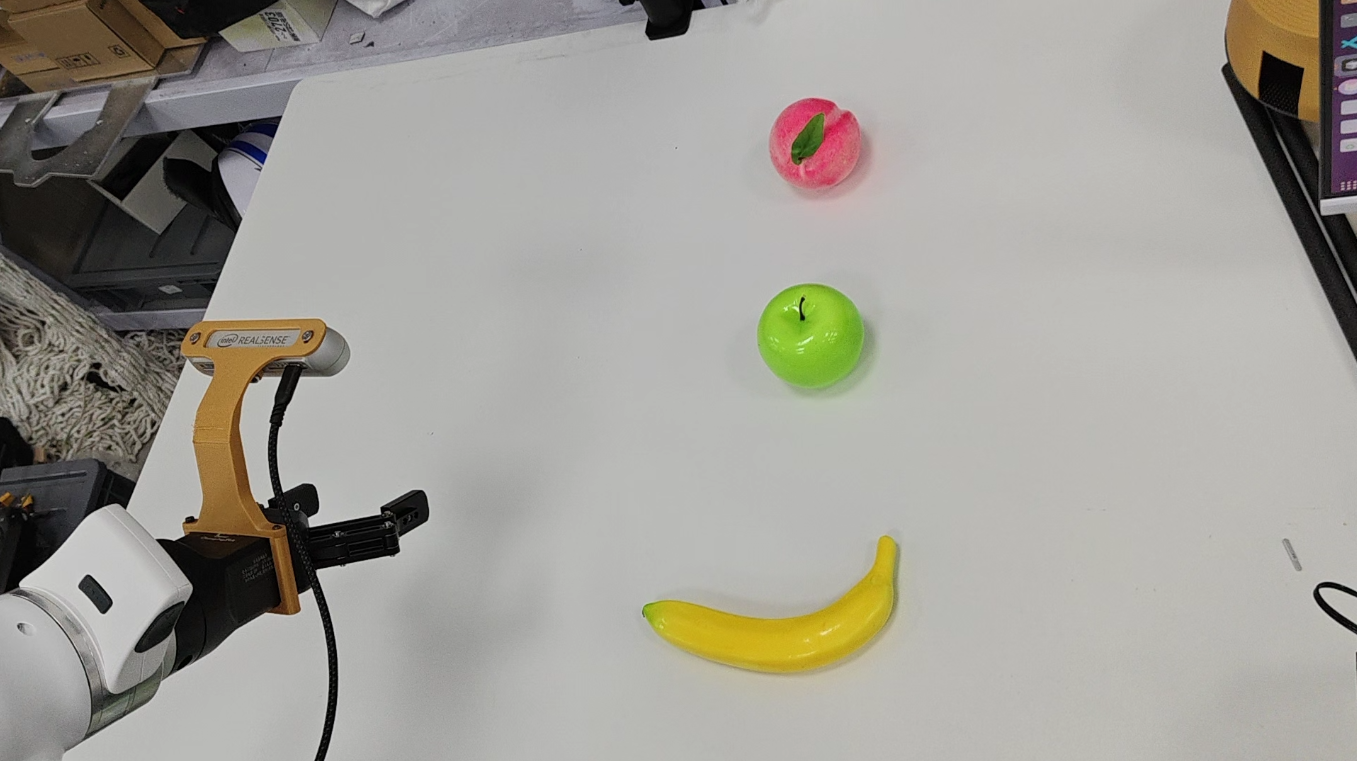
\includegraphics[width=0.30\textwidth]{images/grap_0.png} &
    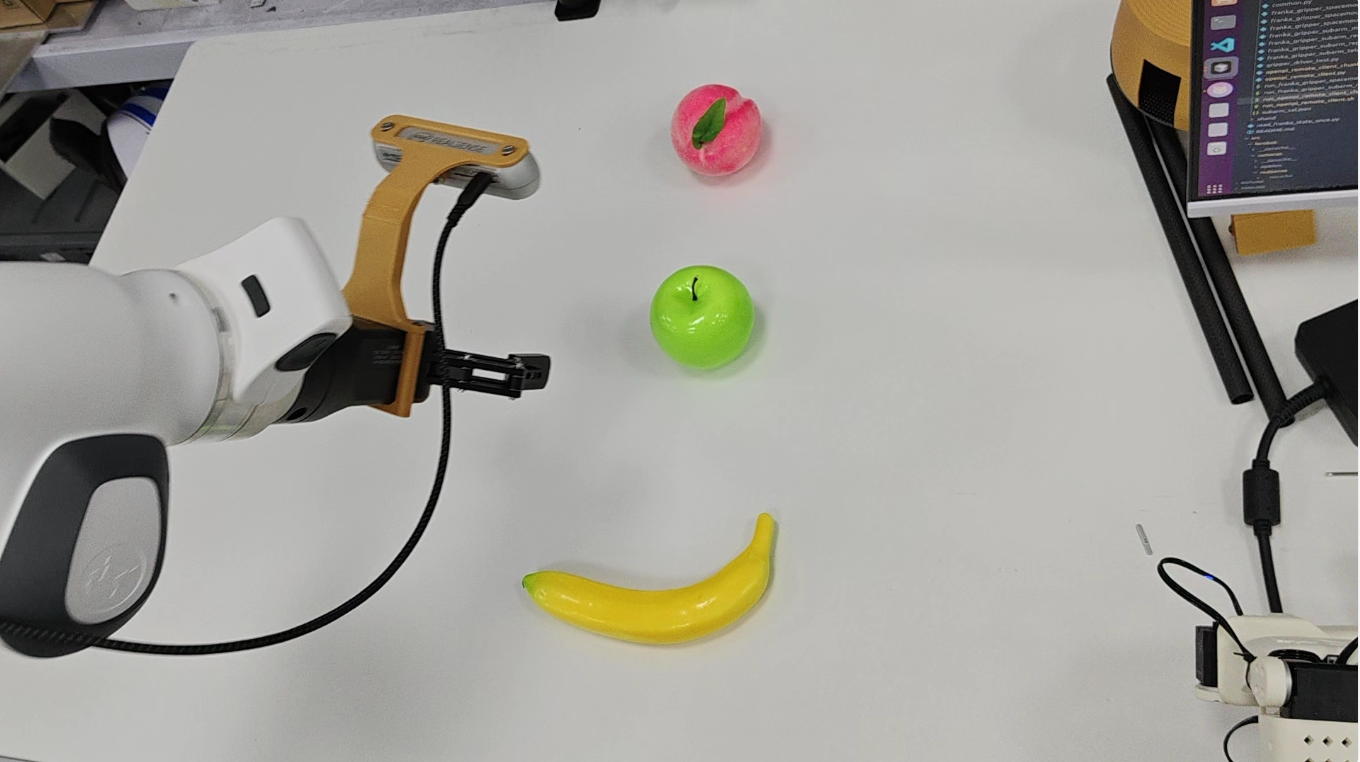
\includegraphics[width=0.30\textwidth]{images/grap_1.png} &
    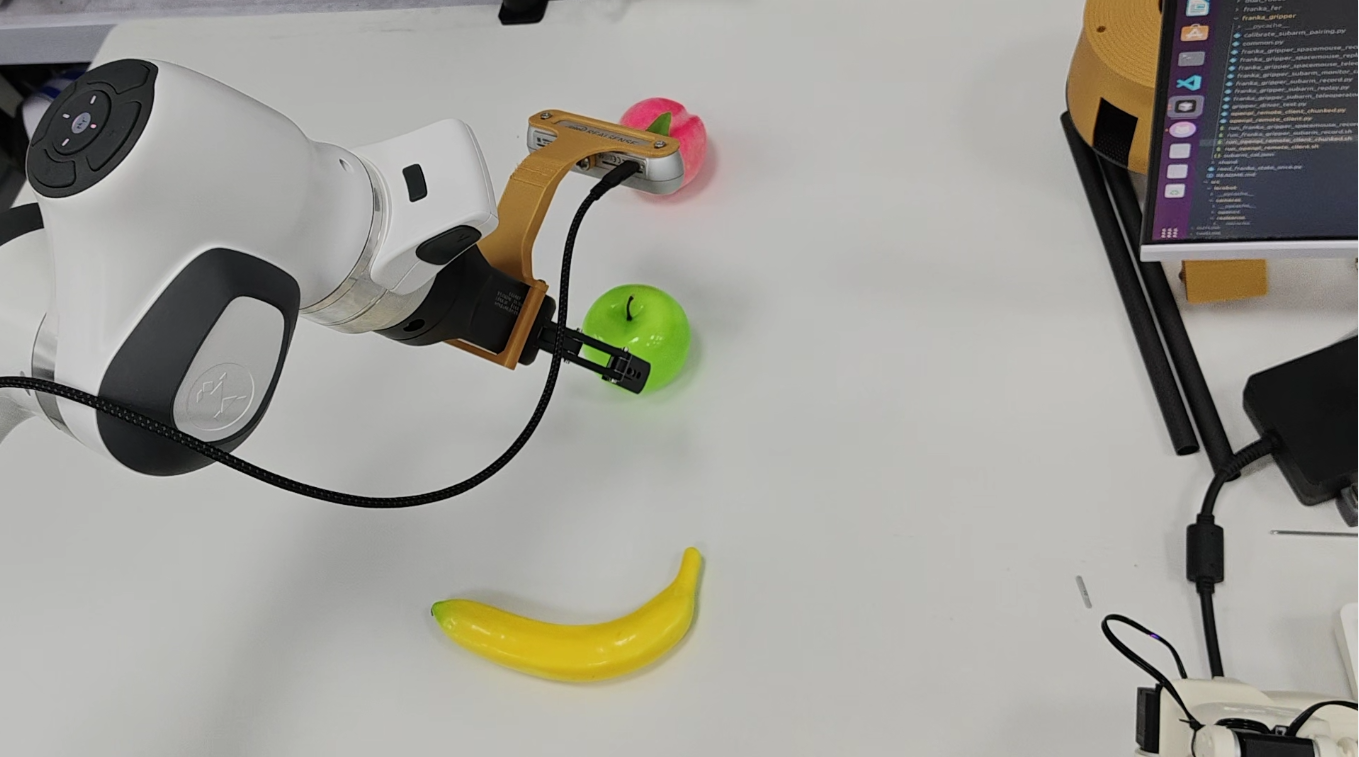
\includegraphics[width=0.30\textwidth]{images/grap_2.png} \\[-2pt]
    \footnotesize 帧30：接近目标 & \footnotesize 帧60：过渡阶段 & \footnotesize 帧90：对准夹取 \\[6pt]
    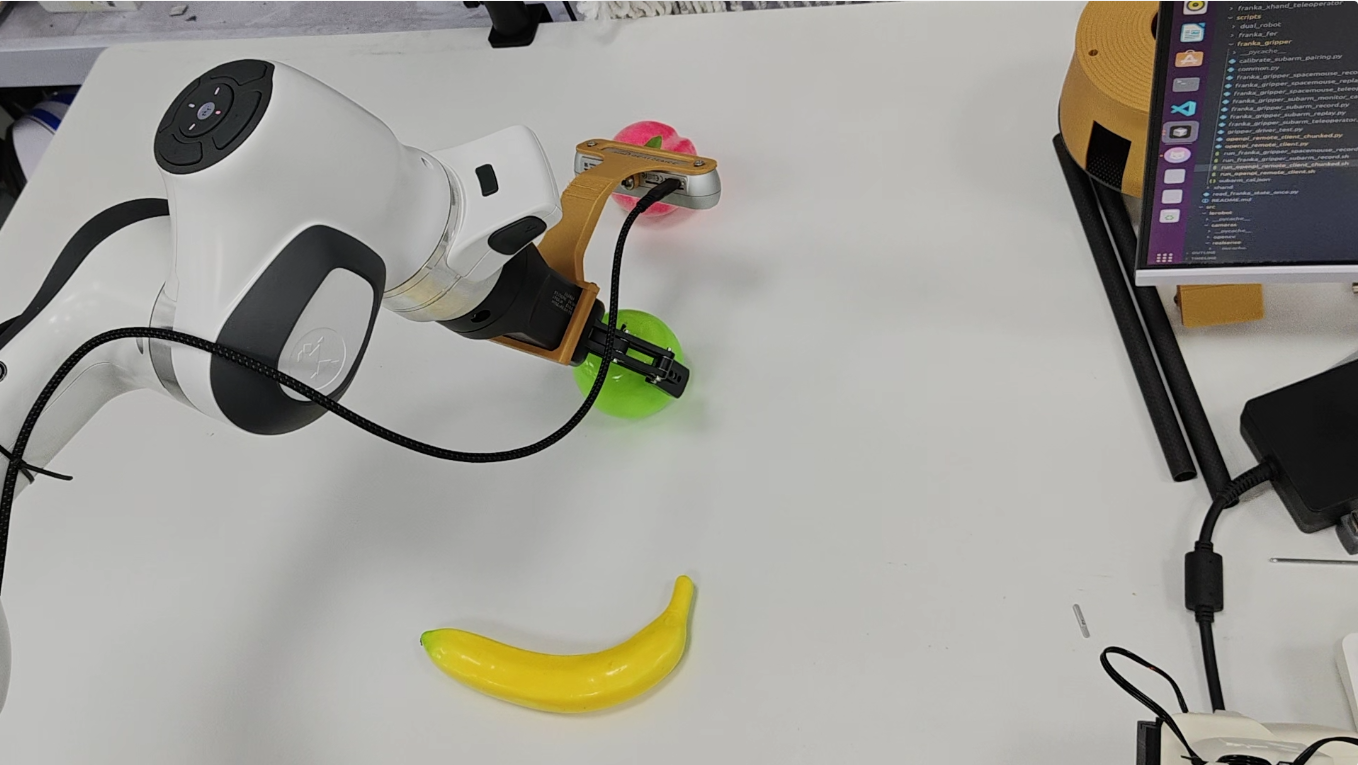
\includegraphics[width=0.30\textwidth]{images/grap_3.png} &
    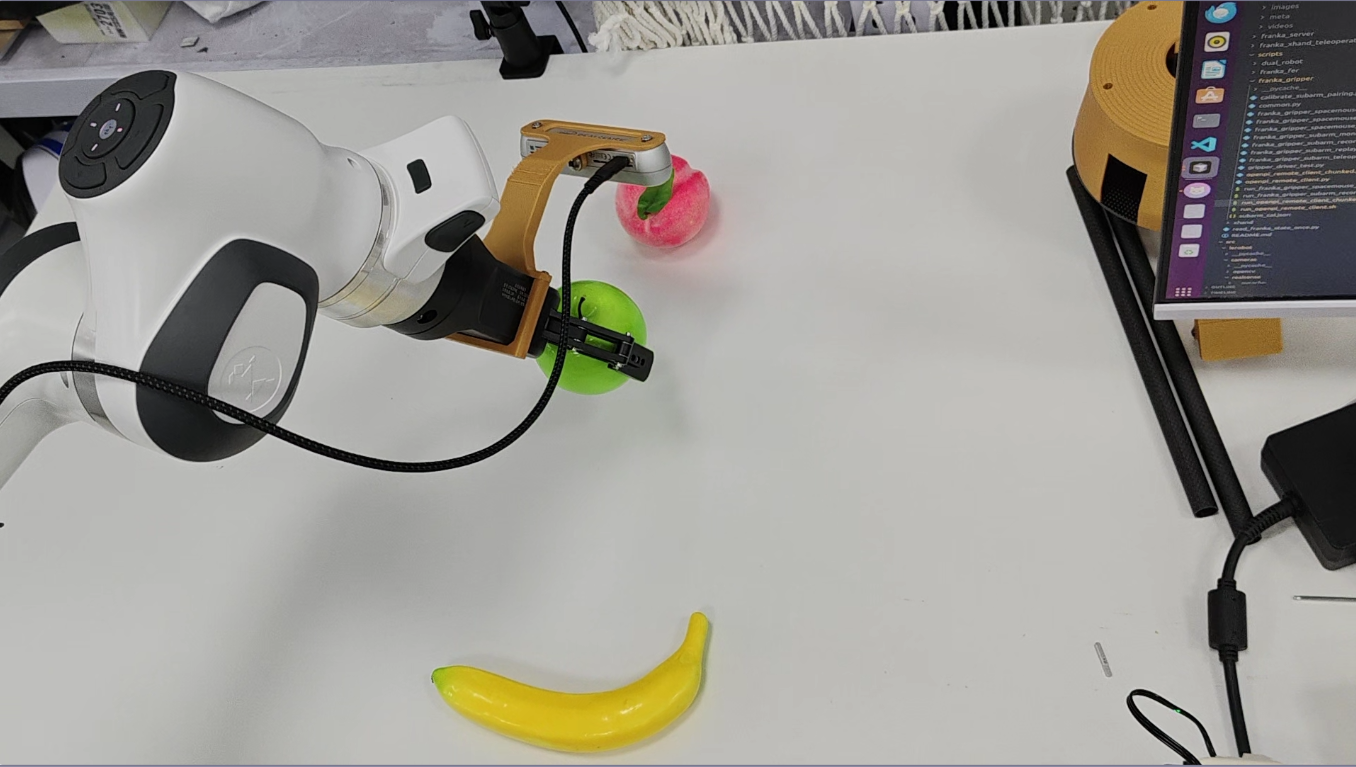
\includegraphics[width=0.30\textwidth]{images/grap_4.png} &
    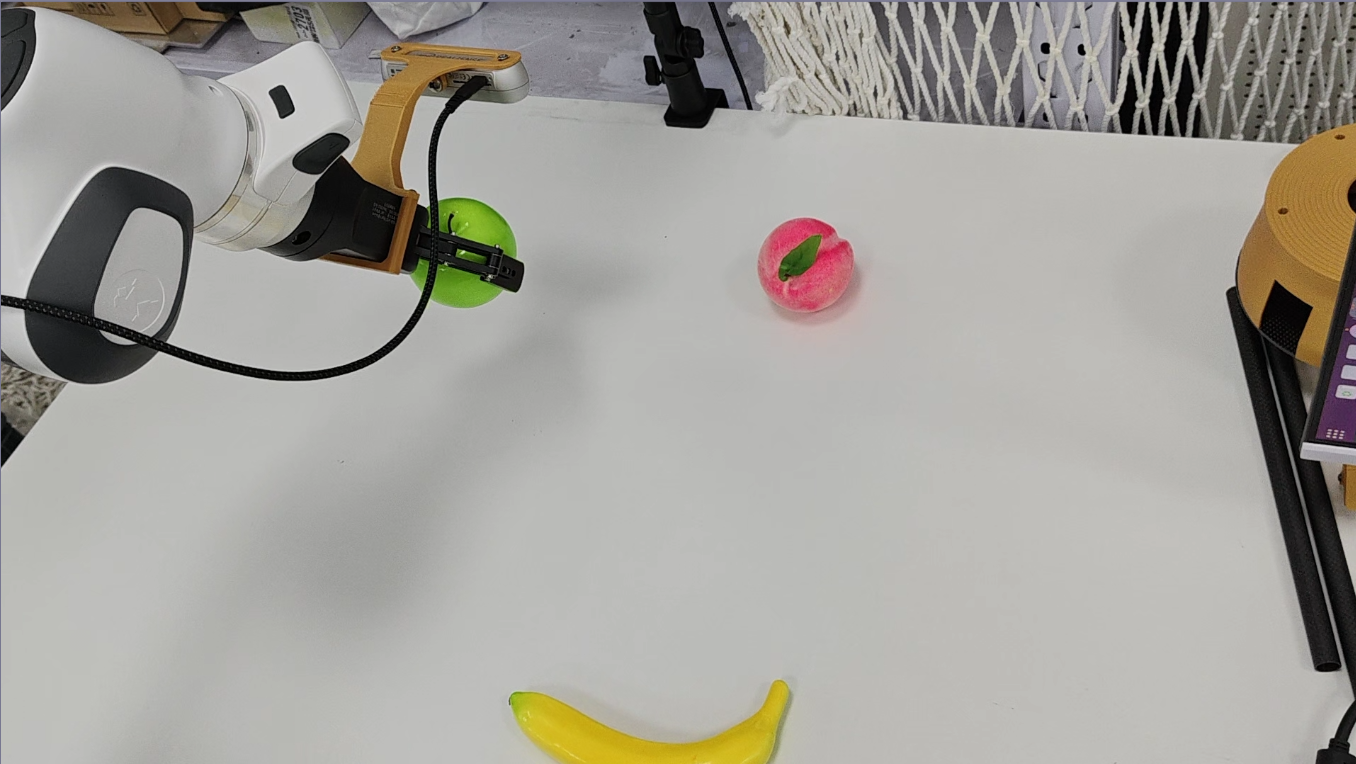
\includegraphics[width=0.30\textwidth]{images/grap_5.png} \\[-2pt]
    \footnotesize 帧120：闭合夹爪 & \footnotesize 帧150：抬升搬运 & \footnotesize 帧180：搬运 \\[6pt]
    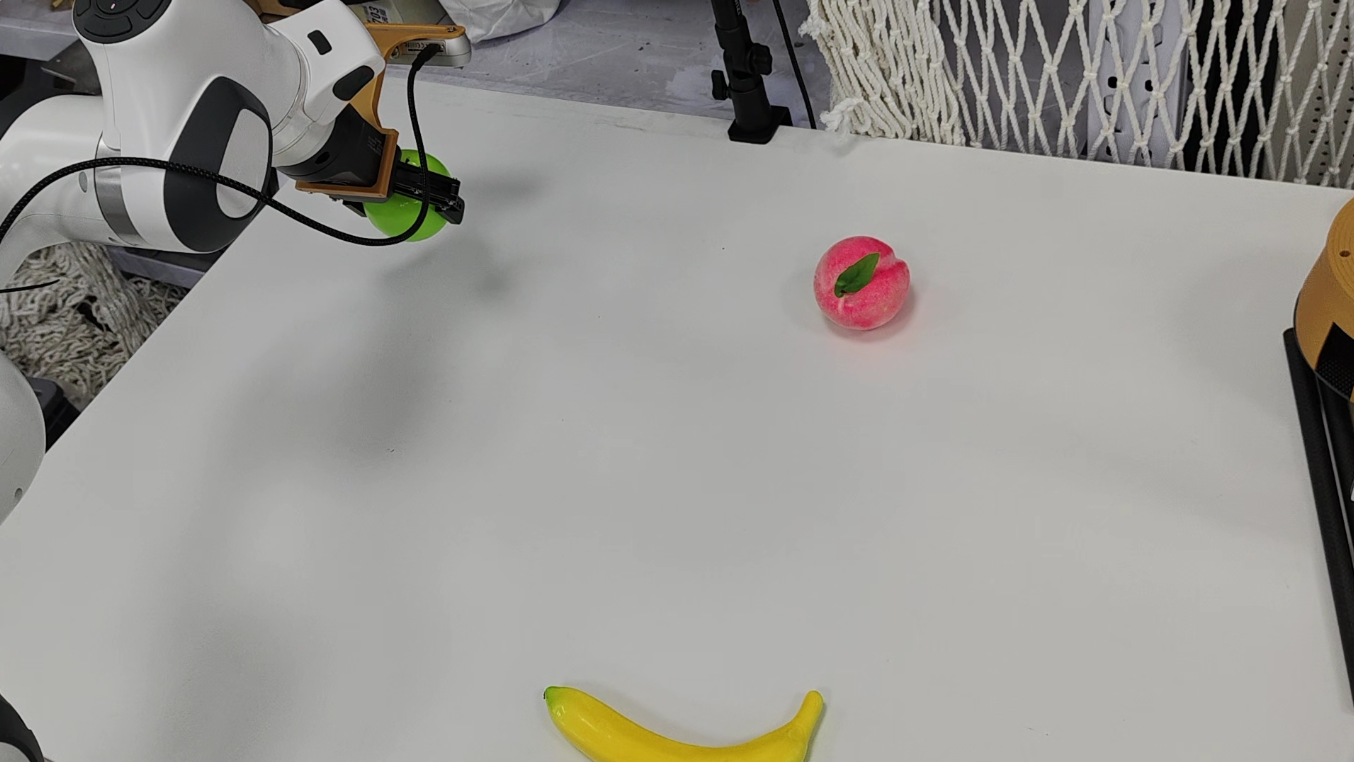
\includegraphics[width=0.30\textwidth]{images/grap_6.png} &
    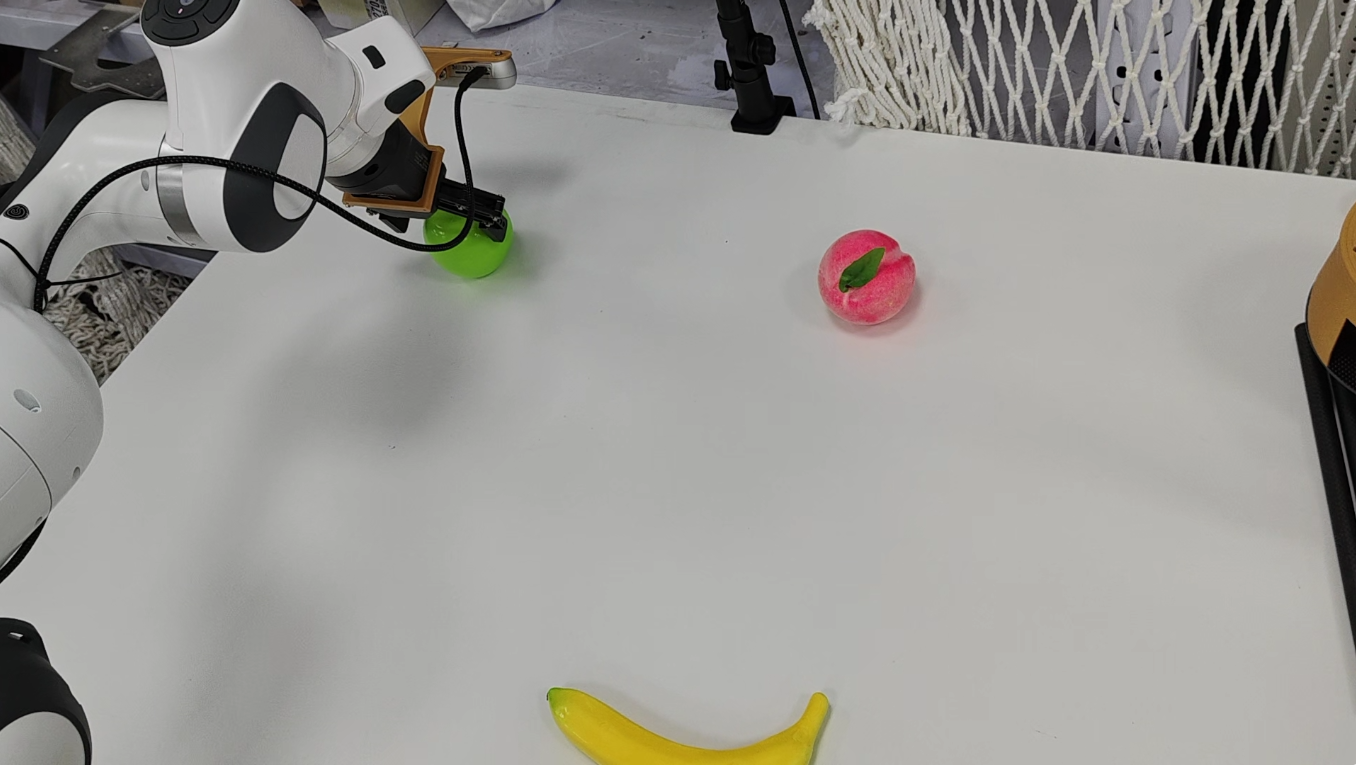
\includegraphics[width=0.30\textwidth]{images/grap_7.png} &
    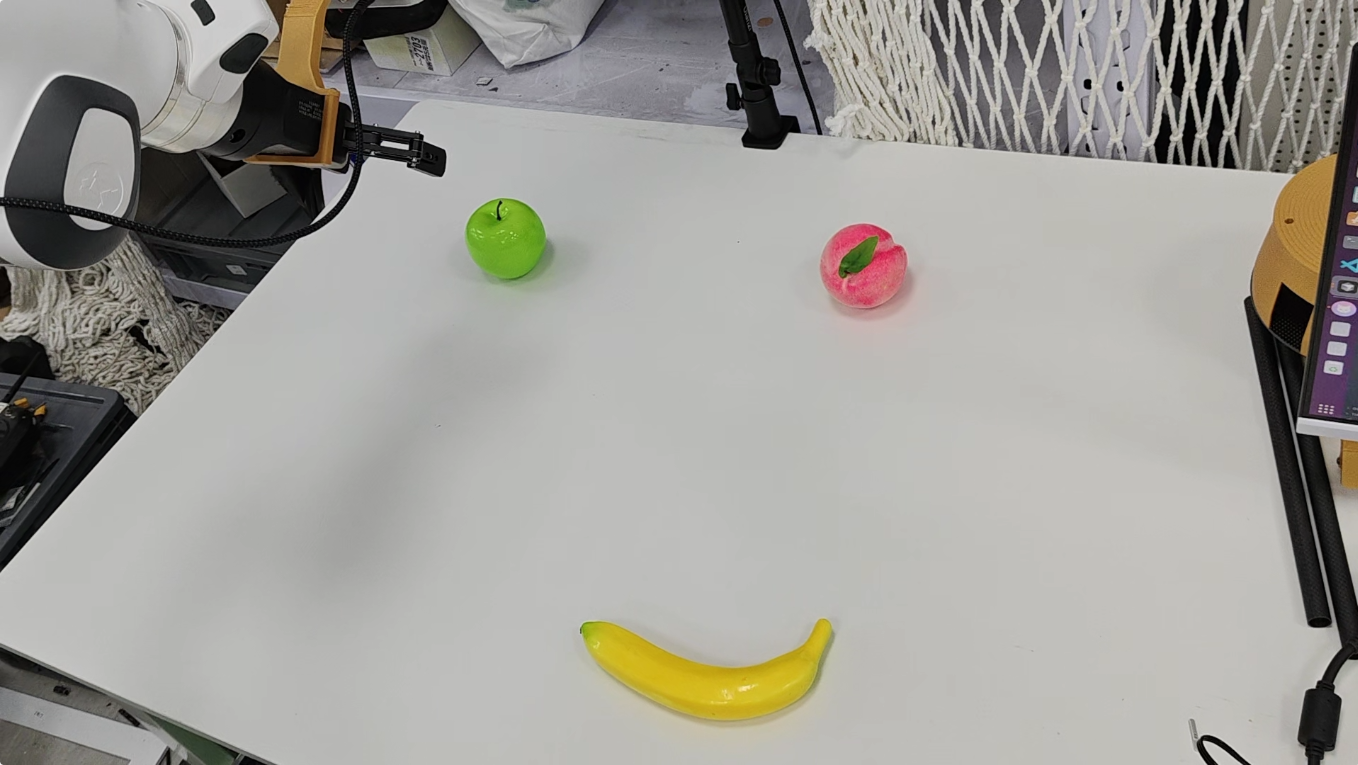
\includegraphics[width=0.30\textwidth]{images/grap_8.png} \\[-2pt]
    \footnotesize 帧210：移至放置区 & \footnotesize 帧240：过渡阶段 & \footnotesize 帧270：释放回撤 \\
  \end{tabular}
  \caption{$\pi_{0.5}$ 实机抓取过程快照}
  \label{fig:vla-grasp-seq}
\end{figure}

\subsection{实验现象与任务完成质量}

从实验现象看，两种部署方式在接近目标与搬运路径平滑性方面都表现出较好的运动质量，
说明训练得到的策略确实学习到了较稳定的桌面抓取动作模式；差异主要集中在抓取接触瞬间及其后的短时稳定保持阶段。
采用异步部署时，机械臂通常能够移动到苹果附近，但夹爪闭合与抬升的配合不够及时，苹果常在指尖边缘滑走，导致任务在最后一步失败。
采用分段闭环部署后，模型可以在每小段执行后重新观察苹果与夹爪的相对位置，因此显著降低了这种接触阶段的误差放大。

这一结果说明，对使用动作块输出的 VLA 而言，部署策略本身与模型结构同样重要。即使训练得到的动作块质量较高，
若部署阶段仍以偏开环的方式执行较长动作序列，实机接触任务也可能出现明显性能下降；而将动作块推理嵌入更紧的闭环中，
往往能够释放模型已有的感知--控制能力。这一结论对于今后将 VLA 部署到高精度桌面装配、插接、对准等任务中也具有普遍意义。

图~\ref{fig:vla-grasp-seq} 给出微调后 $\pi_{0.5}$ 策略在实机在线推理条件下由第三人称相机记录的一组离散画面。
各子图按执行轨迹导出帧序号 $0$--$8$ 排列（自上而下、从左至右），对应同一桌面苹果抓取任务语义下模型闭环执行过程中的若干代表性时刻：
帧0到90 为接近与夹取阶段，帧90到180 为抬升与搬运阶段，帧180到270 为放置与回撤阶段。
与第二章人工示教录制的轨迹不同，此处轨迹完全来自 VLA 根据多相机观测与语言条件逐步推理得到的动作块经实时控制服务执行后的结果；
阶段边界会因推理节拍、动作块截取策略与采样间隔而与连续时间轴略有错位，亦可与腕部视角录像及关节—夹爪时序曲线交叉核对。


\section{全量微调基线性能}
\label{sec:pi05-baseline}

在完成训练配置与部署方式对比后，本文以全量微调版本的 $\pi_{0.5}$ 作为实验基线进行定量评估。该版本在加载 $\pi_{0.5}$ 预训练权重的基础上，对全部参数进行任务特化微调。
在采用分段闭环部署（第\ref{sec:pi05-deploy}节）的条件下，基线模型在 10 次实机抓取测试中成功 8 次，成功率约为 $80\%$，推理显存占用约为 $12\,\mathrm{GB}$，全量微调训练显存约为 160 GB（批次大小为 4）。

全量微调基线的优势在于表达能力完整、上下文利用充分；但其局限性同样明显：数十亿参数的充分更新对仅有 30 条示教轨迹的小样本量而言存在过拟合风险，
且不加约束地更新视觉语言骨干可能破坏预训练中积累的语义先验，反而损害泛化性能。针对这些不足，本文进一步提出了冻结骨干与 短期记忆 两项结构改进，其原理设计、实现细节与实验分析详见第四章。


